\section{Vooronderzoek}

\subsection{wat is een neuraal netwerk}
Neurale netwerken zijn een reeks algoritmen die losjes gemodelleerd zijn van het menselijke brein. Een artificial brein dat gemaalt is uit een hele grote reeks artificial neurons.

\subsubsection{Perceptrons}
Een van de meest fundamenteele artifical neuron type word ook wel een perceptron genoemt en is iest dat je moet weten om een neural network tw begrijpen. Een perceptron pakt verschillende binary inputs:$x_{1}, x_{2},....x_{n}$ en produceerd een enkele binaire output. Je kan het zien als een functie die beslissingen voor je neem door verschillende factoren tegen elkaar te wegen en uiteindelijk met een ja of nee andwoord.
\begin{center}
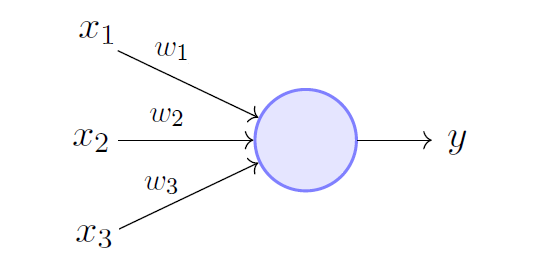
\includegraphics[scale=0.5]{perceptron2.png}
\end{center}
In het voorbeeld hierboven is er een perceptron die 3 variablen als input neemt: $x_{1}, x_{2}$ en $x_{3}.$ Bij all deze waardes word een Weight toegekend($w_{n}$). Deze waarde geeft aan hoe hoe belangrijk die input is voor de neuron. De output van de neuron is de som van alles bij elkaar optellen. $\sum_{j}w_{j}x_{j}$ en deze waarde vegalijken met een gekozen threshold value om de output the brekenen. In een meer wiskundige term:
%\begin{equation*} %tTODO write function
%\begin{rcases}
%        0  if \sum_{j}w_{j}x_{j}+b $\leq$ threshold $\\$
%        1  if \sum_{j}w_{j}x_{j}+b > threshold
%\end{rcases} 
%$\text{output}$
%\end{equation*}
Je kan de output van een neuron beinvloeden door te spelen met de weights en de thresholds.
Door een input's weight te vergroten of de threshold te verlagen kan je een heel ander beslissing model creëren.\\
\newline
Het is duidelijk dat de perceptron niet een compleet model is over hoe mensen hun beslissingen nemen. Maar het voorbeeld illustreert hoe een perceptron verschillende soorten bewijs kan afwegen om beslissingen te nemen. Daarom is het aannemelijk dat een complex netwerk van perceptrons vrij subtiele beslissingen zou moeten kunnen nemen:
\begin{center}
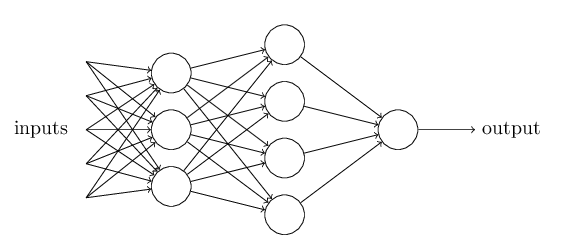
\includegraphics[scale=0.5]{perceptron3.png}
\end{center}
In het netwerk hierboven neemt de eerste laag van perceptrons drie simpelen beslissingen door de hierboven besproken functies uit te voeren. Naast de eerste laag zit er nu ook een tweede die de outputs van de eerste laag als input neemt. Op deze manier kan een perceptron in de tweede laag een beslissing nemen op een complexer en abstracter niveau dan perceptrons in de eerste laag. Deze complexiteit en abstarctheid word verhoogd per extra laag dat je toevoegdt. Op deze manier kan een veellagig netwerk van perceptrons zeer geavanceerde beslissingen nemen.\\
\newline
De volgende stap is om ons netwerk zelf lerend te maken. Om dit te doen moet je kleine aanpassingen kunnen maken aand de weights en de biases. Deze kleine aanpassingen moet daarna ook een klein effect hebben op de output van het neurale netwerk. Echter dat is niet wat er gebeurt met perceptronen want deze heeft maar 2 outputs, een 1 en een 0. Een kleine aanpassing zal daarom niks doen of de hele uitkomst van de perceptron omdraaien. Je kan niet probleem omzeilen door een ander types neurons te gebruiken ,zoals de Sigmoid en tanh neurons.

\subsubsection{tanh neurons}
sigmoid en tanh neurons lijken erg op perceptrons alleen de manier hoe de ouput berekend word is anders. 


\subsection{python}

\subsection{Encog}